\documentclass[12pt,a4paper]{article}
\usepackage[utf8]{inputenc}
\usepackage[english]{babel}
\usepackage[T1]{fontenc}		%imposta la codifica dei font
\usepackage{setspace}
\onehalfspacing
\usepackage{enumitem}
\usepackage[utf8]{inputenc}	%lettere accentate da tastiera
\usepackage{layaureo}	
%\usepackage[margin=1in]{geometry}	%imposta i margini di pagina
\usepackage{multirow}
%\usepackage{graphicx}
\usepackage{amsmath}
\usepackage[final]{graphicx}
\setlength\parindent{0pt}
\usepackage{subcaption}
\usepackage{mathrsfs}
\usepackage{amsfonts}
\usepackage{amssymb}
\usepackage{hyperref}
\usepackage{biblatex}
\usepackage[font=scriptsize]{caption}
\usepackage{algorithm}
\usepackage{algorithmic}
\addtolength{\footnotesep}{2mm}
\DeclareUnicodeCharacter{2212}{-}
\DeclareUnicodeCharacter{2217}{-}
\DeclareUnicodeCharacter{2248}{-}
\DeclareUnicodeCharacter{2261}{-}
\begin{document}
\section{Data Loading and Summary Statistics}

\begin{center}
\begin{tabular}{lccccccc}
\hline
\hline
county &      price &  year built &  sq. feet &  bath &   bed &  rooms &  stories \\
\hline
\hline
Los Angeles     &  311463.93 &     1952.02 &  1602.58 &  1.99 &  3.09 &   7.93 &     1.13 \\
     &  184235.51 &       15.51 &   623.01 &  0.80 &  0.83 &   2.07 &     0.35  \\
 \hline
Orange    &  296527.63 &     1981.45 &  1541.97 &  2.15 &  2.59 &   6.10 &     1.59 \\
     &  175936.36 &        7.82 &   763.17 &  0.67 &  0.91 &   1.52 &     0.52  \\
  \hline
Riverside     &  181315.32 &     1973.89 &  1623.62 &  2.20 &  3.12 &   6.13 &     1.20 \\
 & 105192.13 &       14.58 &   574.24 &  0.67 &  0.80 &   1.37 &     0.40 \\
  \hline
San Bernardino     &  188940.43 &     1979.34 &  1679.67 &  2.15 &  3.24 &   6.51 &     1.36 \\
    &  110151.44 &       18.15 &   624.28 &  0.62 &  0.84 &   1.63 &     0.49  \\
 \hline
Ventura    &  332179.35 &     1978.35 &  1825.55 &  2.34 &  3.34 &   6.64 &     1.49 \\
&  172623.00 &       16.18 &   750.35 &  0.72 &  0.90 &   1.63 &     0.51 \\
\hline
\hline
\end{tabular}
\vspace{1cm}

\begin{tabular}{lccc}
\hline
\hline
county &      violent crime &  property crime &  year sale \\
\hline
\hline
Los Angeles    &         618.81 &         1976.52 &    1999.92 \\
&         277.87 &          602.79 &       4.20\\
 \hline
Orange     &         314.47 &         1414.16 &    1999.94 \\
&         137.58 &          454.10 &       3.93\\
 \hline
Riverside   &         616.38 &         2436.70 &    1999.83 \\
&         278.70 &          825.46 &       4.23 \\
 \hline
San Bernardino       &         567.67 &         2216.86 &    2000.40 \\
&         247.89 &          607.31 &       4.16 \\
 \hline
Ventura    &         335.66 &         1241.45 &    2000.05 \\
 &         153.63 &          336.07 &       4.13\\
 \hline
\hline
\end{tabular}
\vspace{0.4cm}

Figure 1: summary statistics by county for Los Angeles. Standard errors in parenthesis.
\end{center}

\begin{center}
\begin{tabular}{lccccccc}
\hline
\hline
county  &          price &   year built &      sq. feet &      bath &       bed &     rooms &   stories \\
\hline
\hline
Alameda &  398873.12 &     1962.17 &  1672.36 &  2.03 &  3.17 &   6.51 &     1.43  \\
      &  (203825.86) &       (26.42) &   (661.81) &  (0.76) &  (0.88) &   (1.57) &     (0.51) \\
\hline
Contra Costa    &  374582.36 &     1976.76 &  1833.15 &  2.25 &  3.30 &   8.01 &     1.43 \\
   &  215780.05 &       19.49 &   750.57 &  0.71 &  0.91 &   2.07 &     0.50  \\
\hline
San Francisco     &  501817.09 &     1945.13 &  1497.93 &  1.73 &  2.62 &   5.87 &     1.34 \\
   &  256164.63 &       31.10 &   604.25 &  0.81 &  1.01 &   1.87 &     0.56  \\
\hline
San Mateo     &  503715.01 &     1967.17 &  1587.40 &  2.04 &  2.74 &   5.93 &     1.36 \\
    &  270714.95 &       21.51 &   682.83 &  0.75 &  0.99 &   1.91 &     0.50  \\
\hline
Santa Clara     &  464685.42 &     1971.46 &  1662.79 &  2.16 &  3.21 &   6.85 &     1.40  \\
     &  236499.24 &       18.63 &   640.84 &  0.66 &  0.94 &   1.87 &     0.52 \\
\hline
\hline
\end{tabular}
\vspace{1cm}

\begin{tabular}{lccc}
\hline
\hline
county  &    viol. crime &  prop. crime &    year sale \\
\hline
\hline
Alameda &         441.50 &         1971.13 &    2000.35 \\
&         199.81 &          609.14 &       4.22\\
\hline
Contra Costa    &         415.78 &       1898.75 &    2000.56\\
&         277.93 &          599.84 &       4.14\\
\hline
San Francisco    &  586.16 &         2141.65 &    1999.95 \\
&         208.76 &          349.55 &       4.28\\
\hline
San Mateo    &         349.08 &         1713.20 &    2000.26 \\
&         206.92 &         1211.79 &       4.23\\
\hline
Santa Clara      &    322.56 &         1358.68 &    2000.24 \\
&        131.83 &          283.70 &       4.23\\
\hline
\hline
\end{tabular}
\vspace{0.4cm}

Figure 2: summary statistics by county for San Francisco. Standard errors in parenthesis.
\end{center}
\newpage

\section{Bootstrapped Hedonic Price Function}
all for la

\begin{center}
\begin{tabular}{llrr}
\hline
\hline
&         variables &  coefficients &  bootstrapped SE \\
\hline
\hline
&         intercept &    1990918.84 &       1488943.67 \\
&        year built &       -894.40 &          1518.16 \\
&           sq feet &        148.26 &             2.43 \\
&              bath &      18648.53 &           510.92 \\
&               bed &     -24932.01 &           350.35 \\
&             rooms &      -3354.01 &           746.01 \\
&           stories &       -823.54 &           536.50 \\
&     violent crime &       -202.27 &             3.07 \\
&    property crime &          3.72 &             1.51 \\
&     prop crime sq &          0.00 &             0.00 \\
&     year built sq &         -0.03 &             0.39 \\
&        sq feet sq &         -0.00 &             0.00 \\
&          rooms sq &        552.16 &            45.05 \\
&  violent crime sq &          0.07 &             0.00 \\
&            orange &     -12397.88 &          1157.58 \\
&         riverside &    -106479.98 &           789.33 \\
&       sbernardino &    -111110.97 &           686.70 \\
&           ventura &      -8710.83 &           808.16 \\
 &              1993 &      25673.18 &           944.77 \\
&              1994 &       7701.96 &           989.44 \\
&              1995 &      -6538.97 &           994.44 \\
&              1996 &     -13647.49 &           861.54 \\
&              1997 &     -14647.40 &           889.26 \\
&              1998 &      -5470.47 &           752.06 \\
&              2000 &      10791.70 &           838.22 \\
&              2001 &      24638.86 &           795.53 \\
&              2002 &      48895.05 &           857.54 \\
&              2003 &      88477.68 &           935.52 \\
&              2004 &     149860.21 &          1034.25 \\
&              2005 &     201644.40 &          1087.40 \\
&              2006 &     221171.07 &          1121.52 \\
&              2007 &     206244.15 &          1392.85 \\
&              2008 &      77968.59 &          1276.59 \\
\hline
\hline
\end{tabular}
\end{center}

Results for San Francisco
\begin{center}
\begin{tabular}{llrr}
\hline
\hline
&         variables &  coefficients &  bootstrapped SE \\
\hline
\hline
&         intercept &    1990918.84 &       1488943.67 \\
&        year built &      23074.63 &          1600.97 \\
&           sq feet &        234.74 &             3.14  \\
&              bath &       21681.81 &           685.41 \\
&               bed &    -19333.49 &           451.57  \\
&             rooms &       30724.66 &          1190.00 \\
&           stories &      -28404.72 &           580.80  \\
&     violent crime &       -225.17 &             4.04\\
&    property crime &          -82.04 &             1.83  \\
&     prop crime sq &          0.0093&             0.0003 \\
&     year built sq &        -6.27 &             0.41 \\
&        sq feet sq &         -0.001&             0.0007 \\
&          rooms sq &         -1905.39 &            81.40 \\
&  violent crime sq &       0.11 &             0.00  \\
&       contra costa     &    -58350.23 &           598.72 \\
&    san Francisco       &    154457.08 &          1711.49 \\
&     san Mateo           &     92095.40 &          1045.20\\
&      santa clara           &     35950.65 &           560.07 \\
& 1993             &    -46035.24 &          1060.24 \\
& 1994             &    -17405.89 &          1150.96 \\
& 1995             &    -32501.51 &          1147.55 \\
& 1996             &    -43951.30 &          1050.19 \\
& 1997             &    -22901.13 &          1029.56 \\
& 1998             &     -6639.55 &          1028.54 \\
&              2000 &       65691.15 &          1181.33  \\
&              2001 &       80782.58 &          1148.72 \\
&              2002 &      90073.65 &          1106.85 \\
&              2003 &      108304.83 &          1146.75 \\
&              2004 &      166159.28 &          1186.18 \\
&              2005 &    255537.35 &          1203.30  \\
&              2006 &      260548.51 &          1331.91 \\
&              2007 &     240559.32 &          1555.04 \\
&              2008 &      111878.35 &          1786.87 \\
\hline
\hline
\end{tabular}
\end{center}

\section{Rosen Estimates}
\begin{center}
\begin{tabular}{lrr}
\hline
\hline
   &   coefficients &  bootstrapped SE \\
\hline
\hline
const         & -203.0529 &           2.9811 \\
 violent crime &    0.1695 &           0.0025 \\
 income        &   -0.0000 &           0.0000 \\
LA            &  -10.0324 &           3.1447 \\
asian         &   -0.1516 &           0.0221 \\
black         &   -0.4901 &           0.0602 \\
hispanic          &   -0.8726 &           0.0610 \\
\hline
\hline
\end{tabular}
\end{center}

\section{Kernel}

\begin{center}
\begin{figure}[h]
 \caption{Gaussian Kernels for $\chi = 2000$}
  \begin{subfigure}{6cm}
    \centering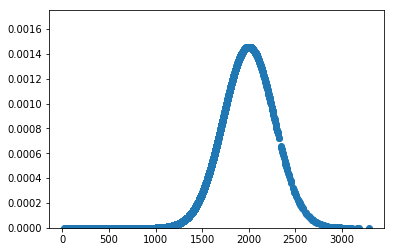
\includegraphics[width=5cm]{gk1.png}
    \caption{$h = 1$}
  \end{subfigure}
  \begin{subfigure}{6cm}
    \centering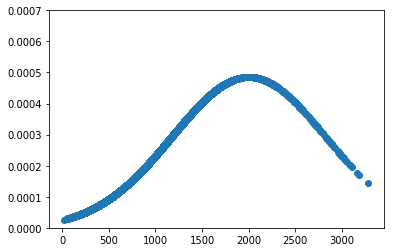
\includegraphics[width=5cm]{gk3.png}
    \caption{$h = 3$}
  \end{subfigure}
 
  \begin{subfigure}{6cm}
    \centering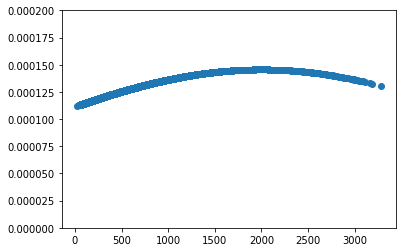
\includegraphics[width=5cm]{gk10.png}
    \caption{$h = 10$}
  \end{subfigure}
  \begin{subfigure}{6cm}
    \centering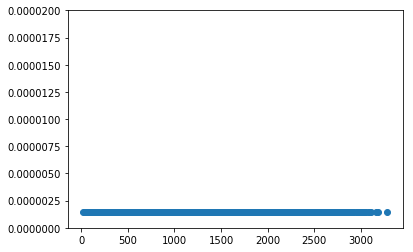
\includegraphics[width=5cm]{gk1000.png}
    \caption{$h = 1000$}
  \end{subfigure}
\end{figure}
\end{center}

\begin{center}
\begin{figure}
 \caption{Hedonic gradients}
  \begin{subfigure}{6cm}
    \centering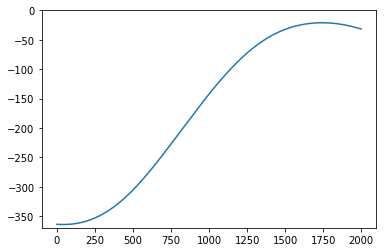
\includegraphics[width=5cm]{b1.png}
    \caption{$h = 1$}
  \end{subfigure}
  \begin{subfigure}{6cm}
    \centering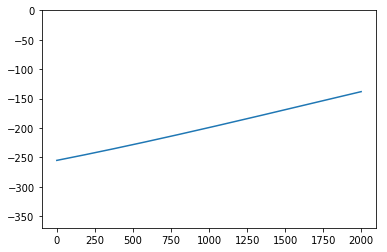
\includegraphics[width=5cm]{b3.png}
    \caption{$h = 3$}
  \end{subfigure}
 
  \begin{subfigure}{6cm}
    \centering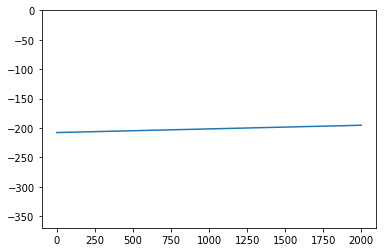
\includegraphics[width=5cm]{b10.png}
    \caption{$h = 10$}
  \end{subfigure}
  \begin{subfigure}{6cm}
    \centering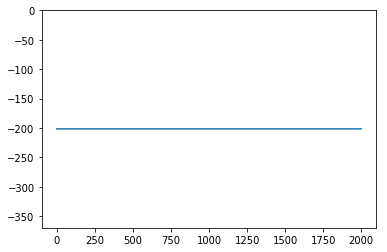
\includegraphics[width=5cm]{b1000.png}
    \caption{$h = 1000$}
  \end{subfigure}
\end{figure}
\end{center}


\end{document}